\documentclass[11pt,a4paper]{jsarticle}
%

\usepackage{amsmath,amssymb}
\usepackage{bm}
\usepackage[dvipdfmx]{color}
\usepackage[dvipdfmx]{graphicx}
\usepackage{ascmac}
\usepackage{listings, jlisting}
\lstset{%
  basicstyle={\small},%
  identifierstyle={\small},%
  commentstyle={\small\itshape},%
  keywordstyle={\small\bfseries},%
  ndkeywordstyle={\small},%
  stringstyle={\small\ttfamily},
  frame={tb},
  breaklines=true,
  columns=[l]{fullflexible},%
  numbers=none,%
  xrightmargin=0zw,%
  xleftmargin=3zw,%
  numberstyle={\scriptsize},%
  stepnumber=1,
  numbersep=1zw,%
  lineskip=-0.5ex%
}


%
\setlength{\textwidth}{\fullwidth}
\setlength{\textheight}{40\baselineskip}
\addtolength{\textheight}{\topskip}
\setlength{\voffset}{-0.2in}
\setlength{\topmargin}{0pt}
\setlength{\headheight}{0pt}
\setlength{\headsep}{0pt}

%
\newcommand{\divergence}{\mathrm{div}\,}  %ダイバージェンス
\newcommand{\grad}{\mathrm{grad}\,}  %グラディエント
\newcommand{\rot}{\mathrm{rot}\,}  %ローテーション
%
\title{チャレンジサイト・メカニックカモノハシ2019\\ micro mouse simulator API}
\author{ER17045 立道壱太郎}
\date{\today}
\begin{document}
\maketitle
%
%
\section*{Mouse}
\subsection*{Mouse( topic\_device, topic\_sensor)}
mouseのコンストラクタです。

\begin{itemize}
\item{topic\_device  }
mouseが配信するTwist型のトピック名を指定します。
初期設定のような物なので、
これは\verb|"cmd_vel"|と指定してください。

\item{topic\_sensor  }
mouseが購読するfloat64型のトピック名を指定します。
初期設定のような物なので、
これはサンプル通りに指定してください。
\end{itemize}


\subsection*{move( fwd, ang, [cnt])}
シミュレータ上のmouseを動かします。

\begin{itemize}
\item{fwd}\\
直進速度[m/s]を指定します。

\item{ang}\\
回転速度[rad/s]を指定します。

\item{[cnt]}\\
実行速度みたいな物です。
デフォルトで10に指定されているので、指定しない場合は10になります。
基本的に指定しないでください。
\end{itemize}


\subsection*{サンプルコード}
\lstinputlisting[caption=script/chapters/1/moving\_mouse.py,label=mouse,numbers=left]{./../../script/chapters/1/moving_mouse.py}




%%%%%%%%%%%%%%%%%%%%%%%%%%%%%%%%%%%%%%%%%%%%%%%%%%%%%%%%%5
\newpage
\section*{wallPublisher}
\subsection*{setData( data)}
\begin{itemize}
\item{data}\\
2次元配列変数を渡してください。
値によってRviz上で壁の色が変化します。

値と色の対応表は以下の通りです。
\end{itemize}

\begin{table}[htb]
  \begin{tabular}{|l|c|l|}
    0 & 透明   & walls.WALL\_INVISIBLE \\
    1 & 白    & walls.WALL\_WHITE \\
    2 & 赤    & walls.WALL\_RED \\ 
    3 & オレンジ & walls.WALL\_ORANGE \\
    4 & 黄色   & walls.WALL\_YELLOW \\
    5 & 緑    & walls.WALL\_GREEN \\
    6 & 青    & walls.WALL\_BLUE \\
    7 & 紫    & walls.WALL\_PURPLE \\
    8 & 灰色   & walls.WALL\_GREY \\
  \end{tabular}
\end{table}

\subsection*{publish()}
Rviz上の壁を更新します。

\subsection*{サンプルコード}
\lstinputlisting[caption=script/chapters/2/wall\_publisher.py,label=wall,numbers=left]{./../../script/chapters/2/wall_publisher.py}

\subsection*{サンプルコードの実行結果}
\begin{figure}[h]
  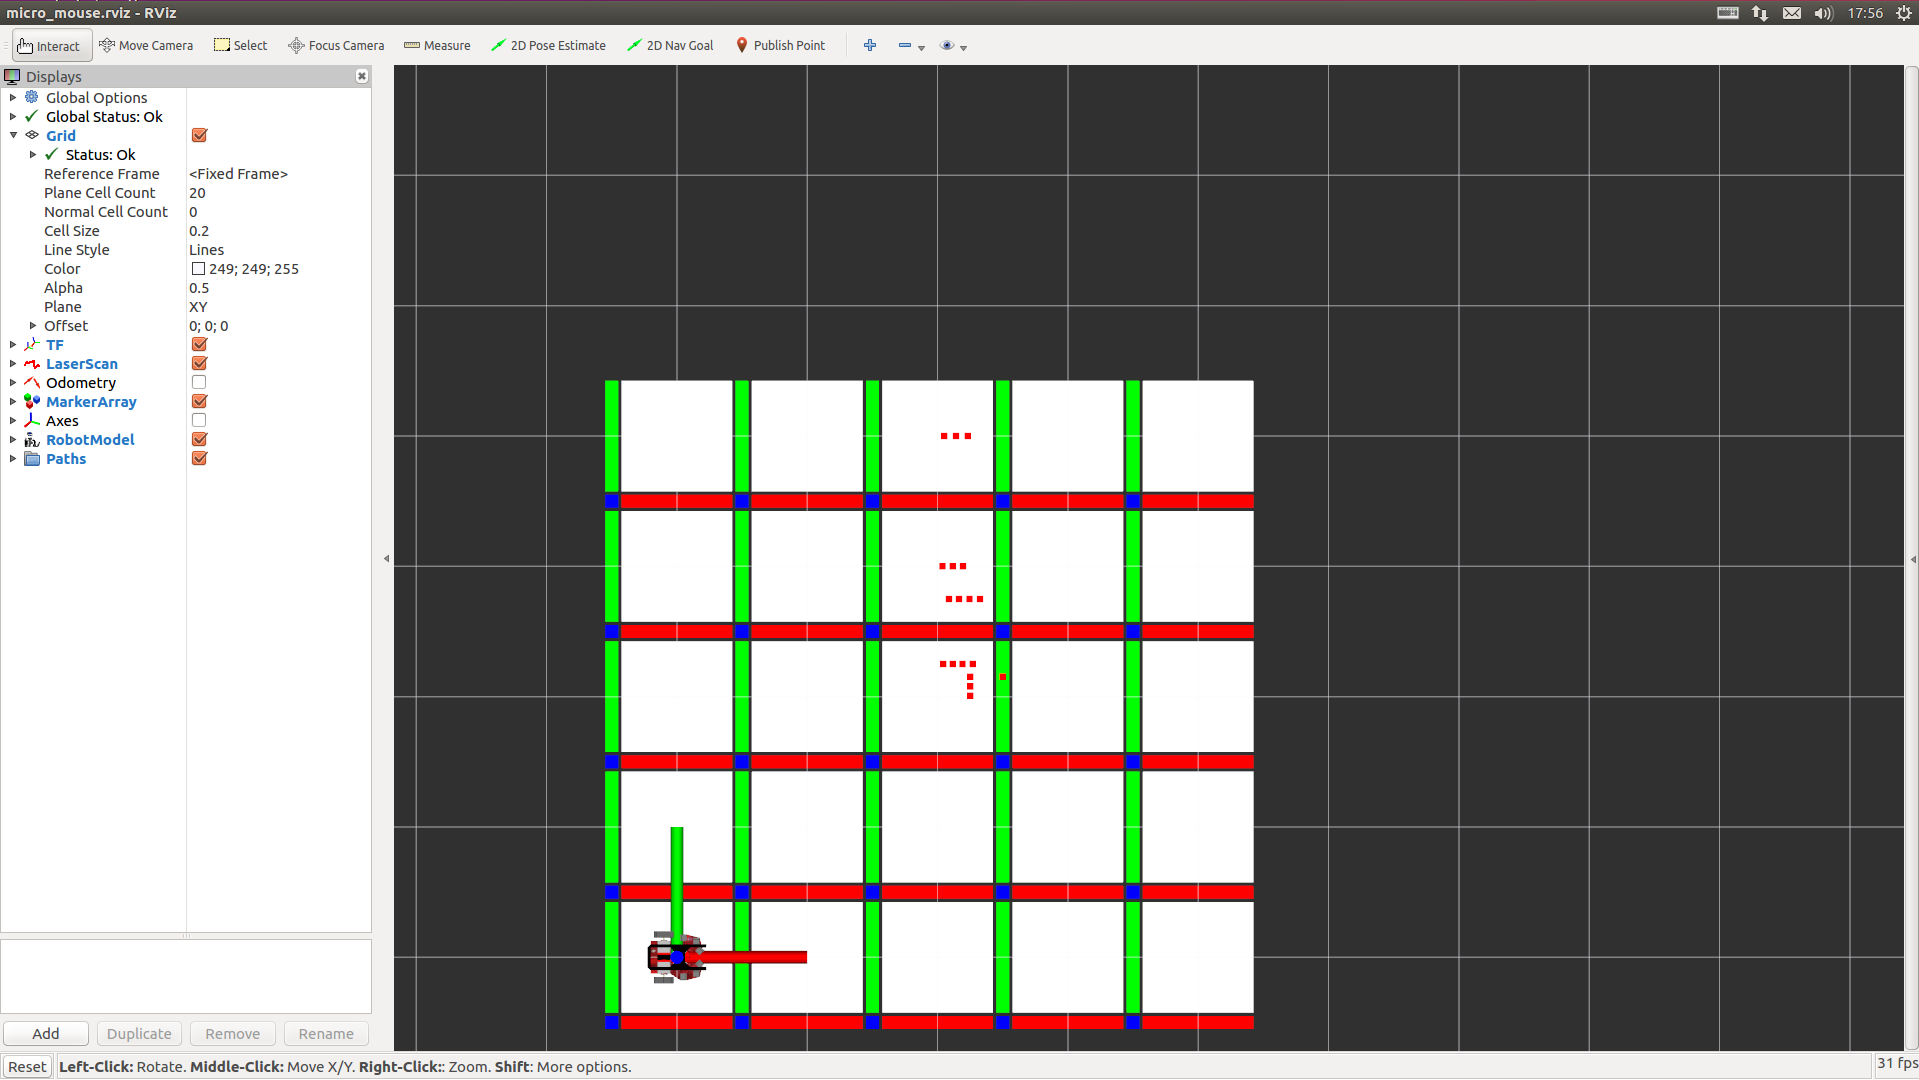
\includegraphics[width=150mm]{./wall_publisher.png}
  \label{wall}
  \caption{wall\_publisher.pyの実行結果}
\end{figure}



%%%%%%%%%%%%%%%%%%%%%%%%%%%%%%%%%%%%%%%%%%%%%%%%%%%%%%%%%5
\newpage
\section*{pathPublisher}
\subsection*{setData( data)}

\begin{itemize}
\item{data}

[[x1, y1], [x2, y2], [x3, y3].....]
というような2次元配列変数を渡してください。
値によってRviz上でpathが変化します。
\end{itemize}

\subsection*{publish()}
Rviz上のPathを更新します。


\subsection*{サンプルコード}
\lstinputlisting[caption=script/chapters/2/path\_publisher.py,label=path,numbers=left]{./../../script/chapters/2/path_publisher.py}

\subsection*{サンプルコードの実行結果}
わかりやすいように色味を変えています。

\begin{figure}[h]
  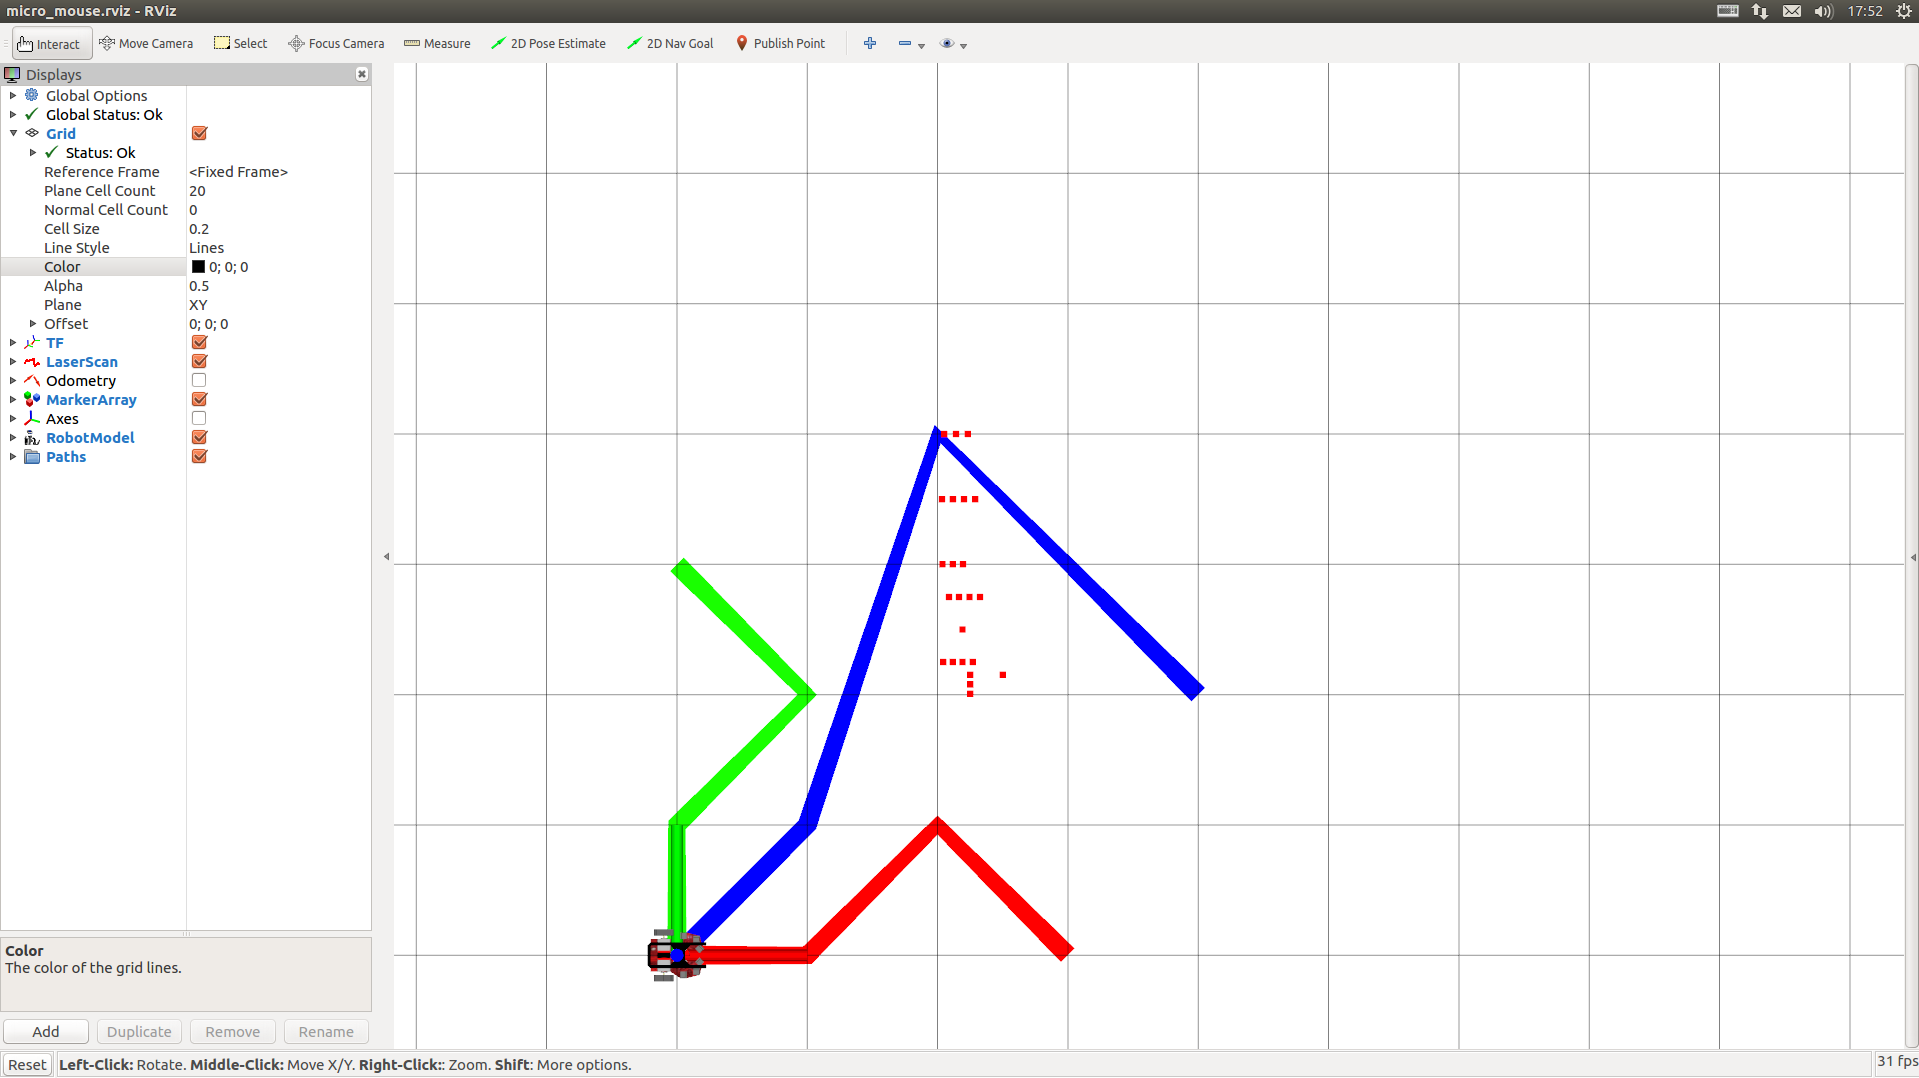
\includegraphics[width=150mm]{./path_publisher.png}
  \label{path}
  \caption{path\_publisher.pyの実行結果}
\end{figure}





%
\end{document}
